\documentclass[10pt,conference]{IEEEtran}

\usepackage{cite}
\usepackage{graphics}
\usepackage{graphicx}
\usepackage{epsfig}
\usepackage{amssymb}
\usepackage{amsthm}
\usepackage{lineno}

\hyphenation{op-tical net-works semi-conduc-tor}

\begin{document}
\title{Ant-based Dynamic Hop Optimization Protocol: a Routing Algorithm for Mobile Wireless Sensor Networks}

\author{
    \IEEEauthorblockN{Alexandre Massayuki Okazaki and Ant\^onio Augusto Fr\"ohlich}
    \IEEEauthorblockA{
        Laboratory for Software and Hardware Integration (LISHA)\\
            Federal University of Santa Catarina (UFSC)\\
            P.O.Box 476, 88040900 -- Florian\'opolis -- Brazil\\
            \{alexandre,guto\}@lisha.ufsc.br
    }
}

\maketitle

\begin{abstract}
In this paper, we introduce Ant-based Dynamic Hop Optimization Protocol (ADHOP), a self-configuring reactive routing protocol for dynamic Wireless Sensor Networks (WSNs).
Our approach is inspired on HOPNET, a multi-hop and self-configuring hybrid routing protocol based on Ant Colony Optimization (ACO) for Mobile Ad Hoc Networks (MANETs).
The ADHOP design considers several restrictions since WSNs tend to be more stringent than MANETs in respect to resource availability, such as energy consumption, processing power, memory, and bandwidth.
There are many challenges in designing routing protocols for WSNs, and topology change is a factor that affects the network lifetime of WSNs.
And with the robustness of routing protocols for MANETs, dealing with dynamic topologies becomes a less arduous task.
Moreover, ADHOP acting together with ACO allows us to deal with the restrictions of WSNs and yet improve the route discovery and the route maintenance through pheromone.
We have evaluated and compared our algorithm to the original HOPNET and obtained better results in terms of data delivery ratio, routing overhead, and congestion avoidance for environments of dynamic topology.
\end{abstract}

\IEEEpeerreviewmaketitle

\section{Introduction}
\label{introduction}

% + Routing on WSNs
%   - problems
WSN consists of a set of sensor nodes which aims at several applications such as home automation, industrial sensing and control, and environment monitoring \cite{Shuang:2009}.
Sensor nodes are characterized by their constraints in processing power, memory, bandwidth, and energy \cite{Matrouk:2009}.
They are often deployed in harsh environments.
As a result, node damage and failure become common events.
Therefore, associated routing protocols must dynamically handle network topology changes.
This adds to the typical topology change of MANETs due to node mobility \cite{Garcia:2007}.
Moreover, by introducing mobility to WSNs, the network capability can be improved in many aspects, such as automatic node deployment, flexible topology adjustment, and rapid event reaction \cite{Wang:2010}.
This way, routing algorithms for WSNs which handle the overhead of topology changes and mobility have attracted a significant interest \cite{Akkaya:2005}.

Several solutions monitor the quality of links using metrics such as signal strength, data reception ratio, location, and heuristics to maintain reliable links between nodes \cite{Stankovic:2008}.
As a result, many routing techniques attempt to obtain routes through reliable links.
Routing algorithms inspired by ACO can be an effective way to deal with dynamic topologies due to the ability of ants to perceive changes in networks through pheromone.

% + Paper goal
In this paper, we introduce a new routing method based on dynamic hops.
It allows us to deal with the overhead of dynamic topologies taking into account congestion and unreliable links between nodes.
We also designed ADHOP, a self-configuring reactive routing protocol that uses the dynamic hops to improve the routing decisions.
ACO-based routing protocols usually provide the ability to learn the shortest routes \cite{Lu:2004} and yet automatically adapt to network topology changes \cite{Iyengar:2007}.
Such routing algorithms have been considered as an alternative for many scalable multi-hop networks, including WSNs \cite{Okdem:2009, Dhurandher:2009}.
Our approach aims at efficiency in data delivery ratio as well as minimizing the traffic overhead.
It helps us to handle important routing problems in ad hoc networks such as route discovery and broken routes.
These contributions allow us to achieve a routing algorithm powerful enough to ensure reliable routes among nodes to handle congestion in dynamic topology environments like MANETs.
However, several routing schemes of MANETs are inadequate for WSNs due to typical limitations of sensor network nodes \cite{Okdem:2009}.
Hence, these constraints were taken in consideration in the architectural design of our routing algorithm in order to achieve a suitable protocol for WSNs.

% + Paper organization
The remainder of this paper is organized as follows: section \ref{related} presents related work.
In section \ref{proposed}, we explain and describe ADHOP.
Section \ref{evaluation}, we evaluate our implementation.
Finally, we present our conclusion of the study in the last section.

\section{Related Work}
\label{related}

The main challenges of routing in WSNs are to support data communication while trying to prolong the lifetime of nodes' batteries, prevent connectivity degradation, decrease congestion, improve energy efficiency.
However, differently from our proposal, most of these protocols do not consider dynamic network topologies.

Vlajic and Stevanovic \cite{Vlajic:2009} analyzed the pros and cons of deploying path-constrained mobile sinks in real IEEE 802.15.4 networks.
They introduced two simple mechanisms for the reduction of mobility-related overhead in WSNs.
They also demonstrated analytically and through simulation that in idealist networks, mobile sinks can result in a better distribution of routing load and longer network lifetime.
Unfortunately, in real world networks, including IEEE 802.15.4, the overhead is not zero.
These networks use mechanisms that generate additional overhead to manage congestion, lessen mobility, and consequently bring down the amount of changes in network topology.
Hence, for contemplating the use of real WSNs with continuous changes in network topology, the minimization of protocol overhead may have to be the first course of action.

% + What is HOPNET?
HOPNET is a self-configuring and multi-hop hybrid routing algorithm for MANETs \cite{Wang:2009}.
It has features extracted from ZRP \cite{Haas:1997} and involves ACO \cite{Dorigo:2006} to solve routing problems.
ZRP is a hybrid routing protocol which aims to reduce the control overhead of proactive protocols and the latency of reactive protocols.
Each node maintains a reactive routing among zones and a proactive routing within its zone to obtain reliable link information between neighbor nodes.
However, HOPNET uses ant collective intelligence in the proactive routing to maintain and improve existing routes or explore better options.
HOPNET has obtained efficiency and good results in terms of data delivery ratio and overhead for networks of high scalability and high mobility.

\section{ADHOP: The Proposed Routing Strategy}
\label{proposed}

% + Section goal

ADHOP is an evolution from \emph{Ant-based Dynamic Zone Routing Protocol} (AD-ZRP) \cite{Okazaki:2011}, a routing protocol which uses pheromone as a metric to make routing decisions within dynamic zones.
ADHOP is also a self-configuring and multi-hop reactive routing protocol inspired on HOPNET.
With the robustness of HOPNET, it handles important problems in mobile networks.
The idea behind routing protocols based on ACO is to apply the behaviour of ants in the network to discover and maintain the best routes among nodes.
These protocols can thereby maintain the routing table updated efficiently due to the proportionate dynamism of ants to detect, by pheromone, changes in the network topology.

In HOPNET, source nodes can quickly obtain a route to any destination that shares the same zone.
However, if most of the transmissions are to nodes outside the zone, then the routing becomes expensive.
For instance, if the external node is not in the routing table as a destination, but it is part of any route, then each route has to be verified minutely in order to find this node.
The source node could also start a search process in order to discover a new route to the external node.
Anyway, both processes waste memory, processing, and bandwidth.

In order to reduce the on-demand data transmissions, HOPNET allows us to increase the zone radius.
Nonetheless, defining an optimal zone radius for each network is a challenge.
Different from HOPNET, which uses fixed-sized zones defined by a zone radius, our approach abstracts the concept of zones and focus on the next hop that the ant has to perform.
ADHOP aims to minimize the latency while reducing the network overhead.
Each node in ADHOP can store an amount of pheromone between itself and any other node in the network.
All routing decisions are made locally, without needing to know a entire route to transmit data.
In order to make routing decisions properly, the ants are responsible for dissipating the knowledge of the network thus teaching to nodes the best route to be taken at that instant.
Therefore, nodes do not need to be concerned to discover and maintain entire routes.
They just need to direct the data to the next hop toward the destination node through a local decision.

The routes in ADHOP are not predetermined and the hops are chosen dynamically at each node toward the destination.
This way, our approach adapts to topology changes and network needs transparently, as shown in Figure \ref{dynamic}.
In Figure \ref{dynamic} (a), from the source to a particular destination, the ADHOP algorithm define the best route by pheromone.
In Figure \ref{dynamic} (b), a node fails along the route.
Meanwhile, this part of the route is no longer used, then the other nodes eventually leaves the route due to pheromone evaporation.
The same happens when one of the nodes moves away from the route, as shown in Figure \ref{dynamic} (c).

\begin{figure*}[htb]
\centering
\begin{tabular}{c c c}
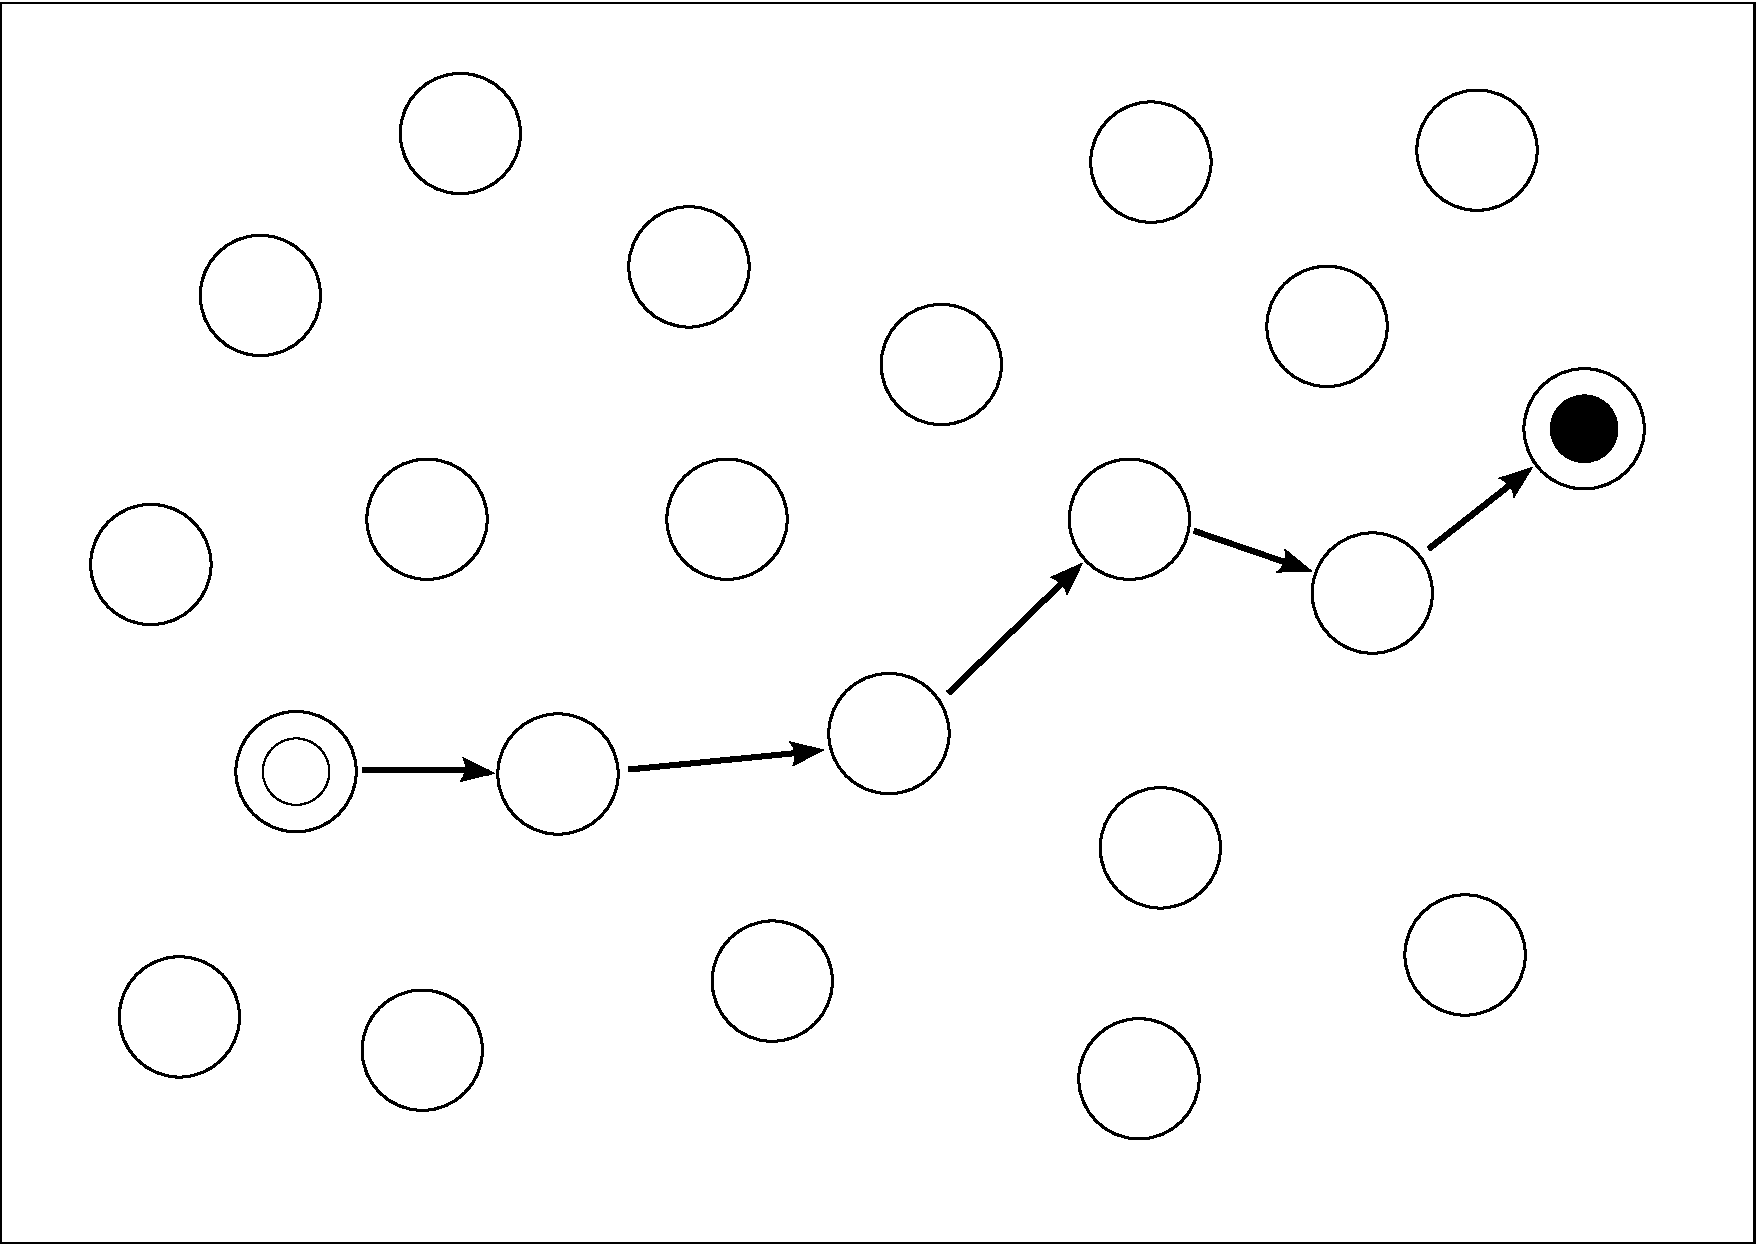
\includegraphics[width=134pt]{fig/dynamic_1.pdf} &
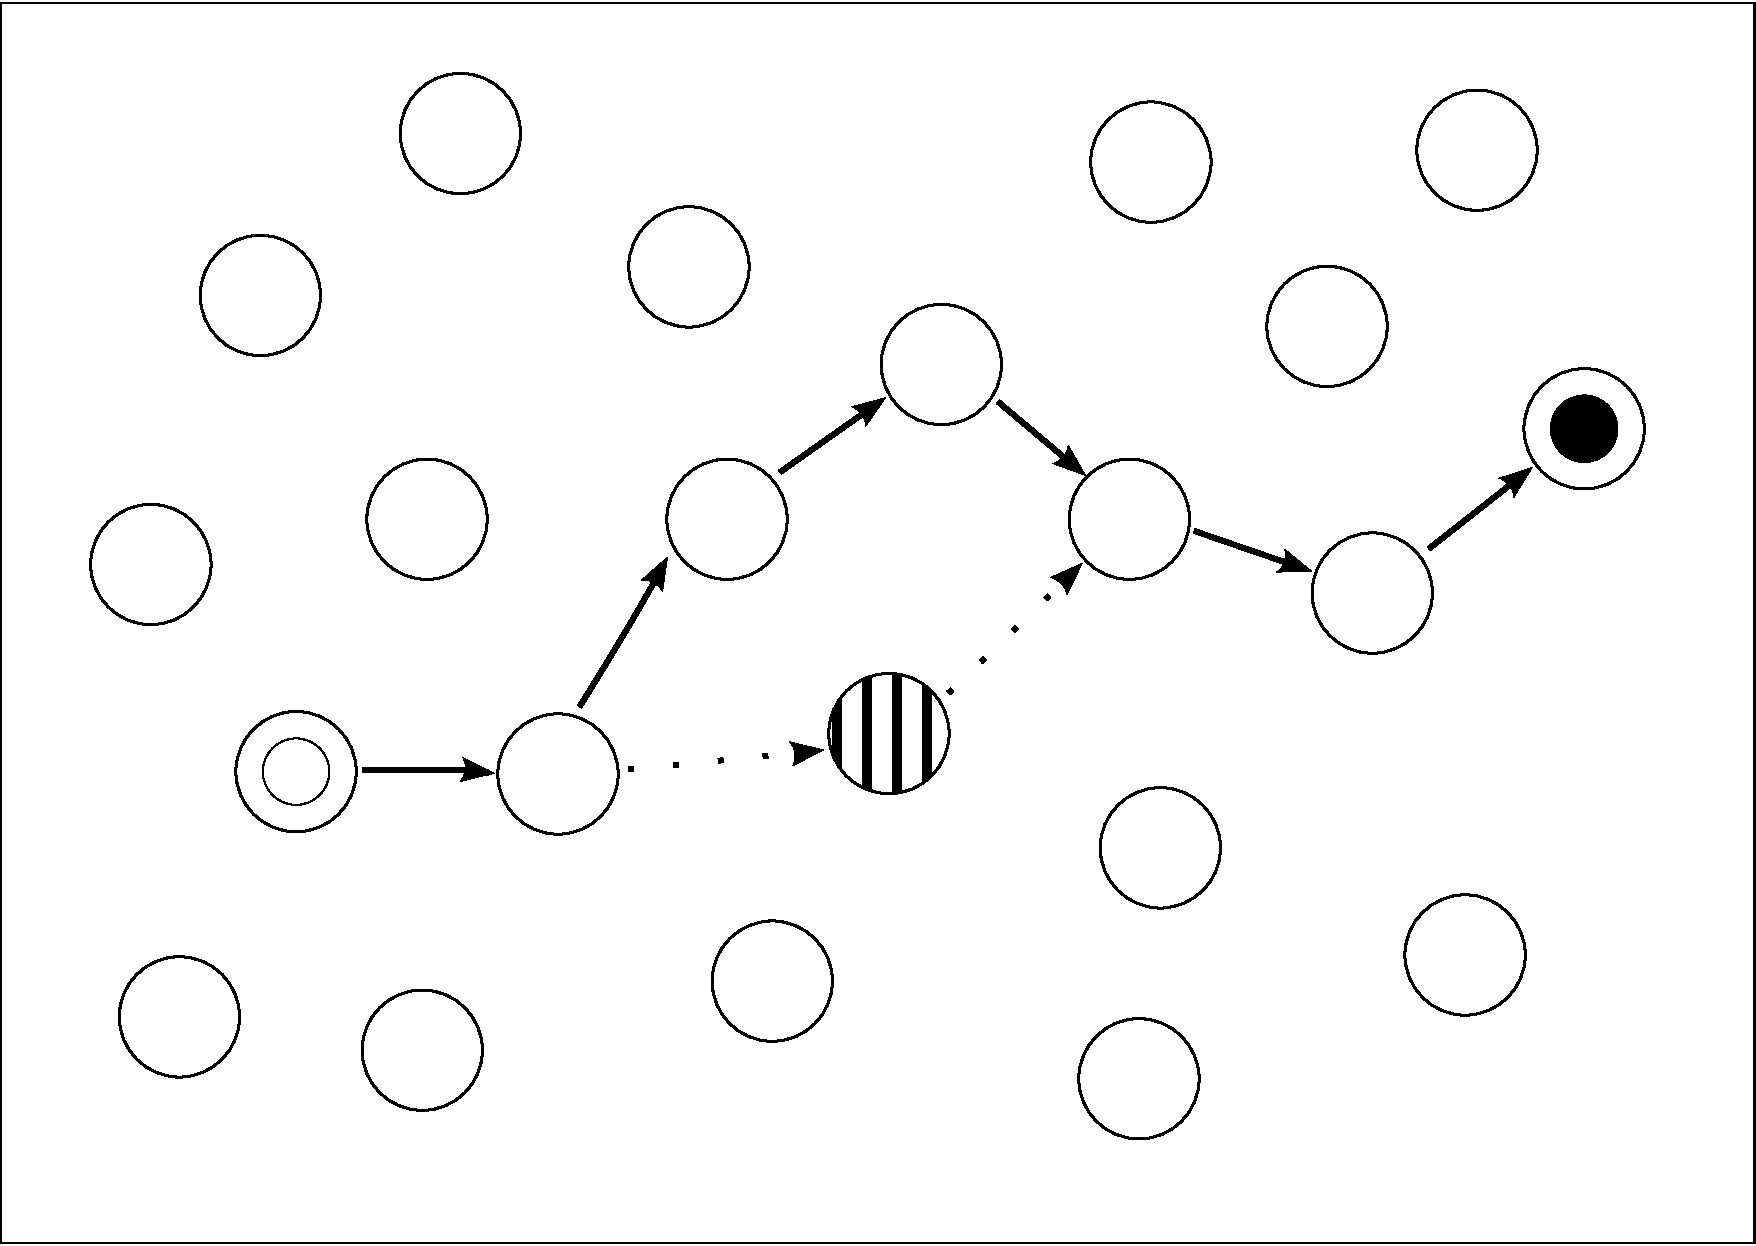
\includegraphics[width=134pt]{fig/dynamic_2.pdf} &
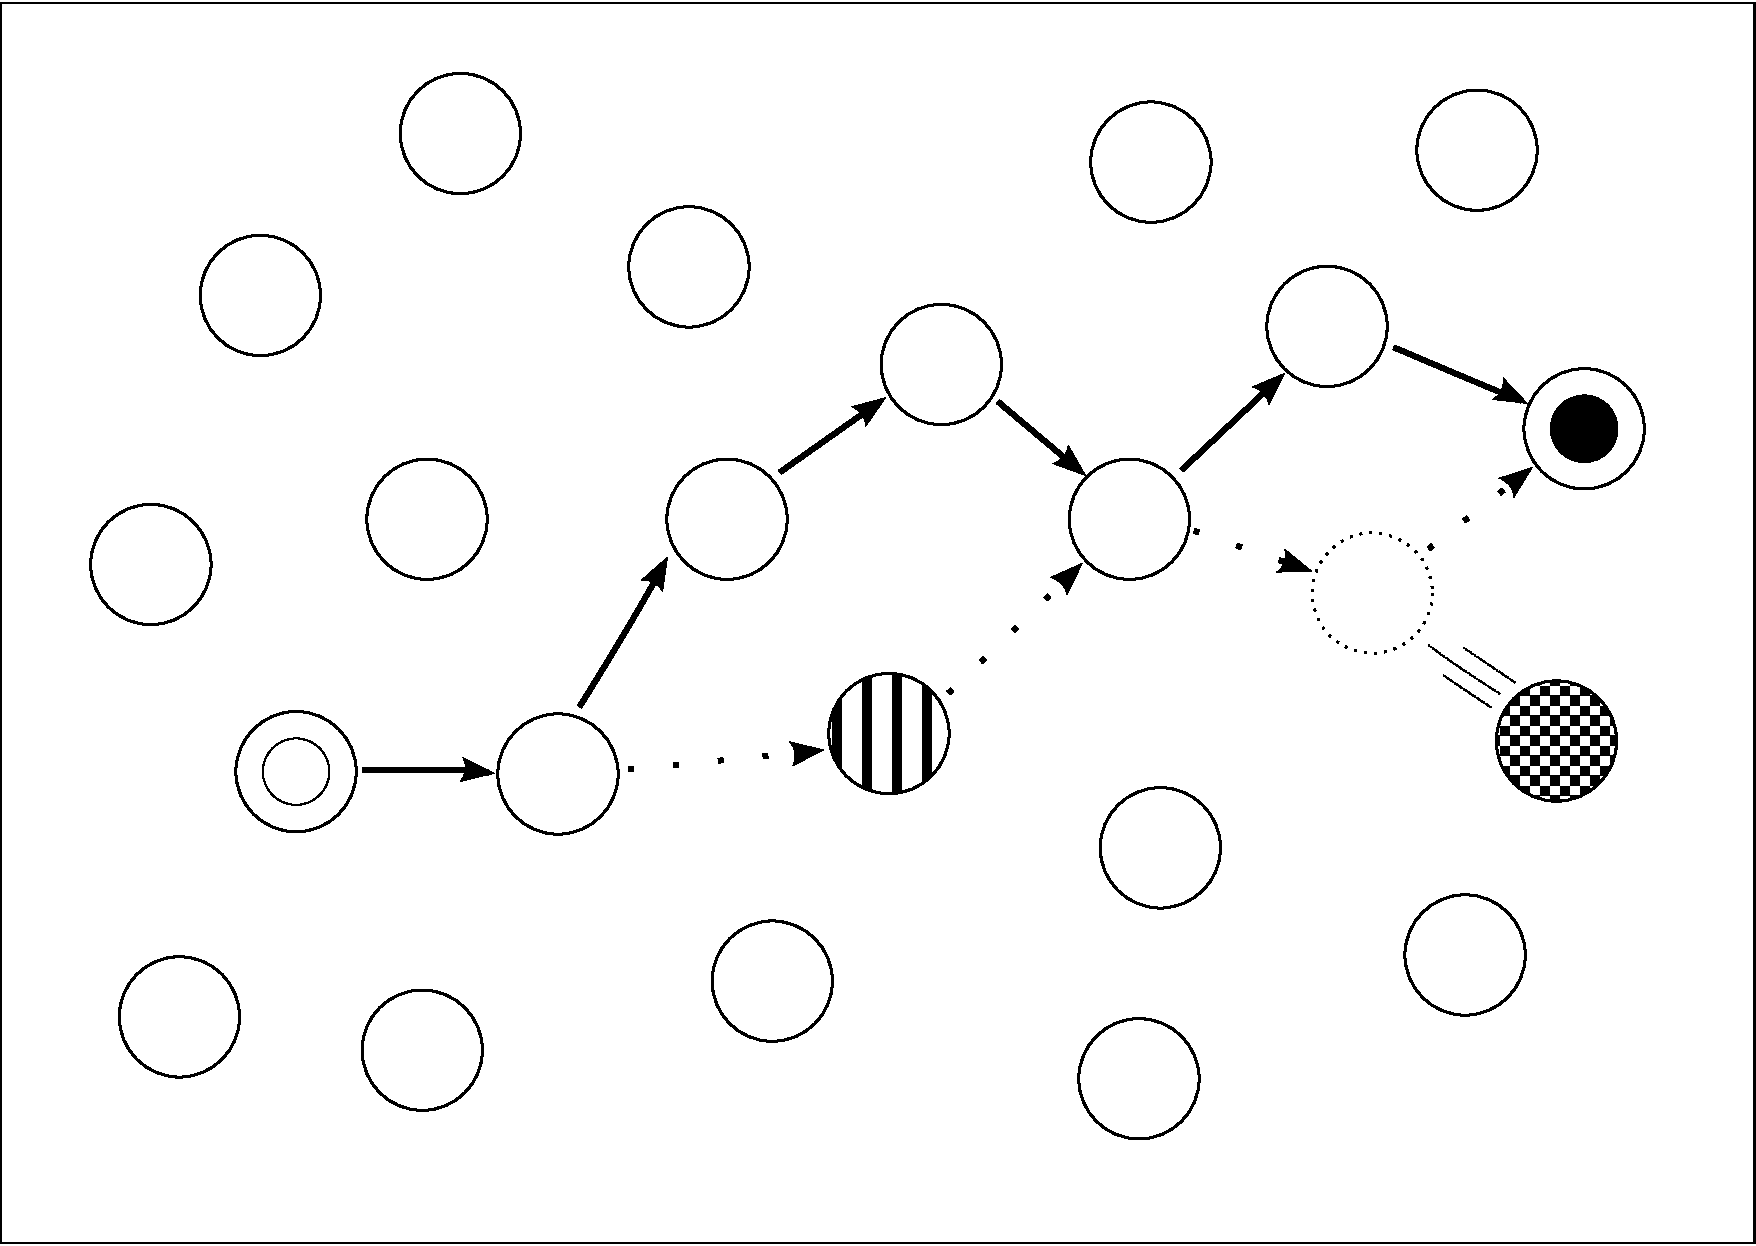
\includegraphics[width=134pt]{fig/dynamic_3.pdf} \\
\multicolumn{3}{c}{ 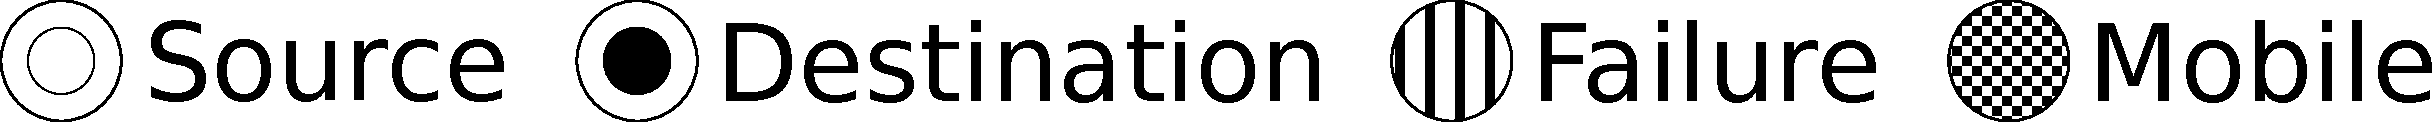
\includegraphics[width=200pt]{fig/dynamic_subtitle.pdf} } \\
(a) & (b) & (c) \\
\end{tabular}
\caption{Dynamic Hops}
\label{dynamic}
\end{figure*}

In order to accomplish these routing operations, a new collection of ants is presented: \emph{forward transport ant} (FTA) and \emph{exploratory transport ant} (ETA).
Although each ant category has a different function, they share a common data structure.
Figure \ref{adhop_protocol} shows the ant data structure of ADHOP.
The data structure includes address fields as \emph{Source} and \emph{Destination}.
The \emph{Previous} field is responsible for storing the address of the previous node.
The \emph{SequenceNO} field is used for control.
The \emph{Type} field indicates the ant category, and the \emph{Hops} field indicates the number of hops which the ant has done.
The \emph{Heuristic Inf.} field is responsible for storing the necessary heuristic information to calculate the evaporation and the pheromone deposit ratio.
These ants help to reduce the complexity by offering better tactics to diffuse and verify pheromone among nodes.
Hence, they reinforce the links between neighbors to maintain the best routes according to the heuristic information.

\begin{figure}[htb]
\centering
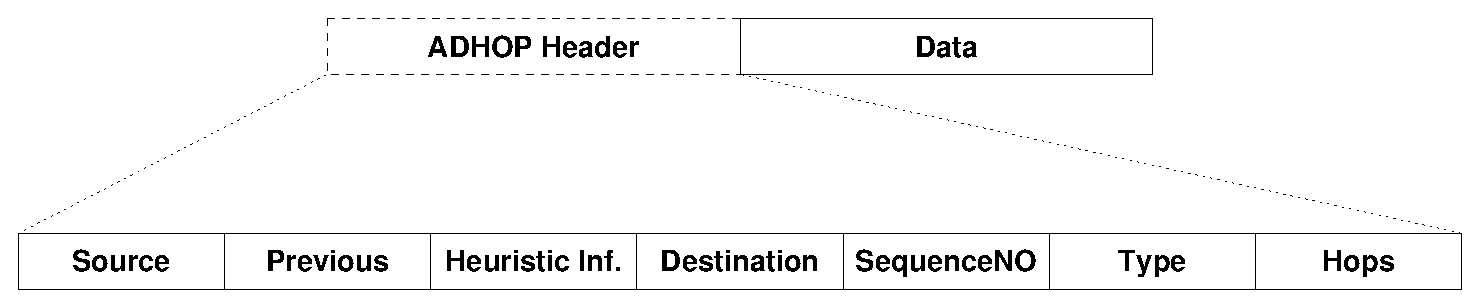
\includegraphics[width=220pt]{fig/adhop_protocol.eps}
\caption{ADHOP Ant Structure}
\label{adhop_protocol}
\end{figure}

In HOPNET, if there is any change in the route during data transmission, ants are sent to notify the other nodes and get a new route respectively.
In ADHOP, the data packet is sent along with the ant to ensure that sudden changes in the network do not interfere with the transportation of the data towards the destination.
The data packet may thereby be dynamically redirected to a safer route.
Figure \ref{adhop_data_tx} depicts the sequence diagram for data transmission in ADHOP.

\begin{figure}[htb]
\centering
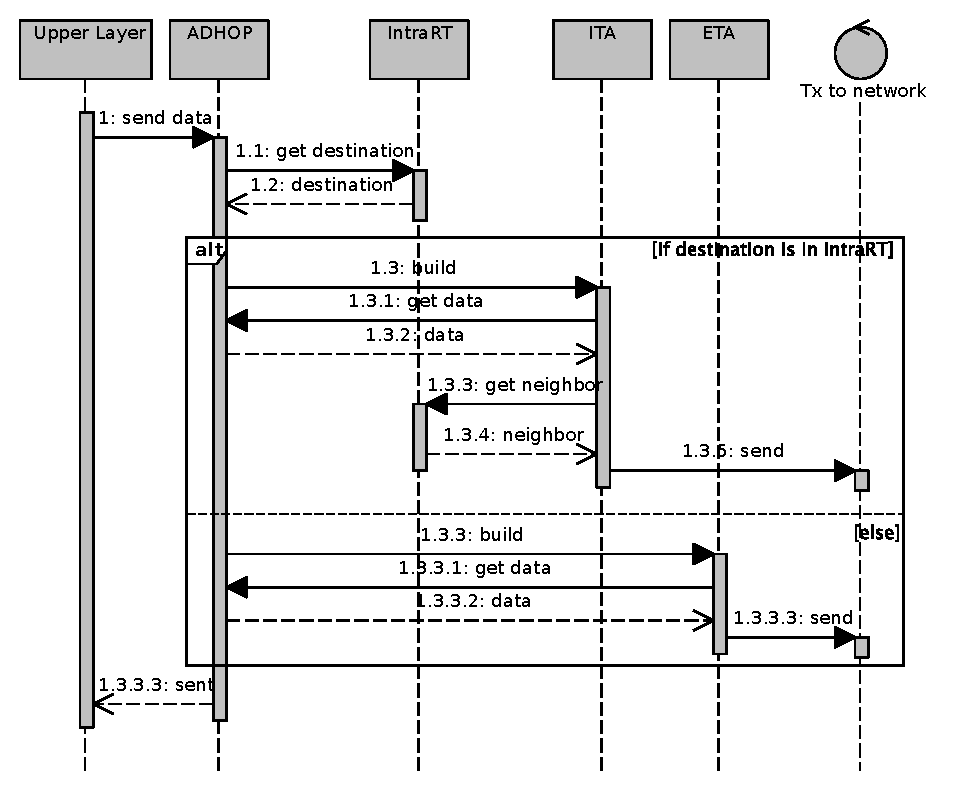
\includegraphics[width=220pt]{fig/adhop_data_tx.eps}
\caption{ADHOP - Data Transmission}
\label{adhop_data_tx}
\end{figure}

ETAs are responsible for discovering routes to unknown nodes.
These ants travel through the network to discover the destination node.
At the destination, the ETA delivers the data packet and returns to the source node.
On the way back, the ant just sets the pheromone trail in order to reinforce the route, as shown in Figure \ref{adhop_rx_eta}.

\begin{figure}[htb]
\centering
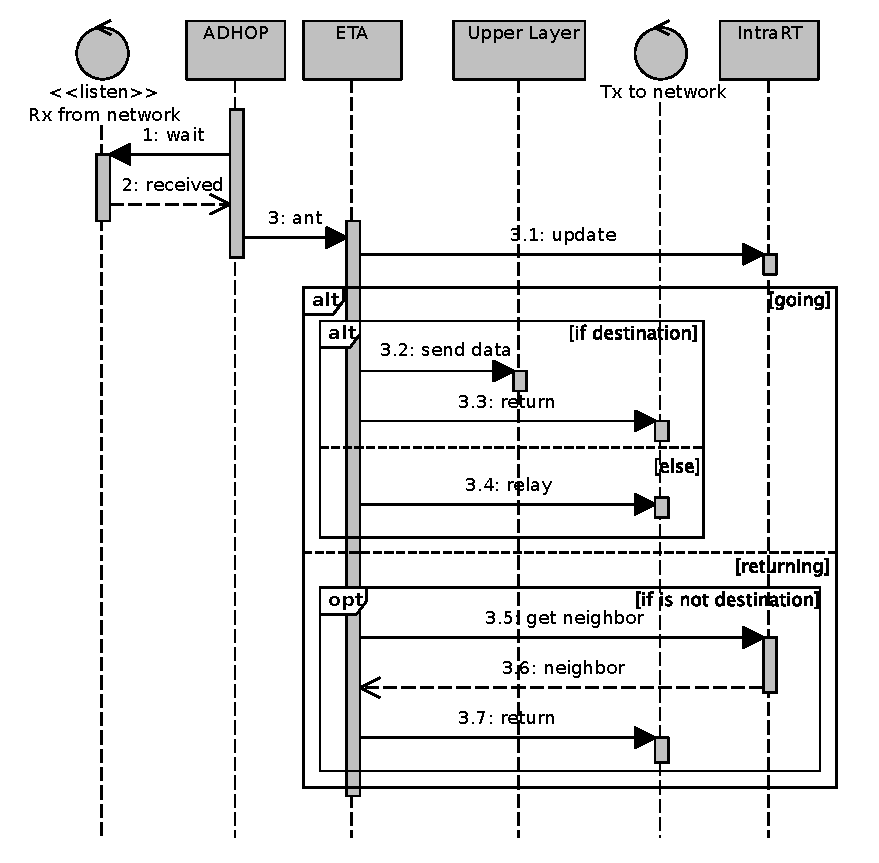
\includegraphics[width=220pt]{fig/adhop_rx_eta.eps}
\caption{ETA Rx}
\label{adhop_rx_eta}
\end{figure}

When a source node discovers a new route to certain destination by ETA, the following data packet transmissions are performed by FTAs until the pheromone amount on the route evaporates entirely.
Nevertheless, at any time, if any route to any destination breaks, any node on the route can use a new ETA to recover it or discover a new path, as the sequence diagram shown in Figure \ref{adhop_rx_ita}.

\begin{figure}[htb]
\centering
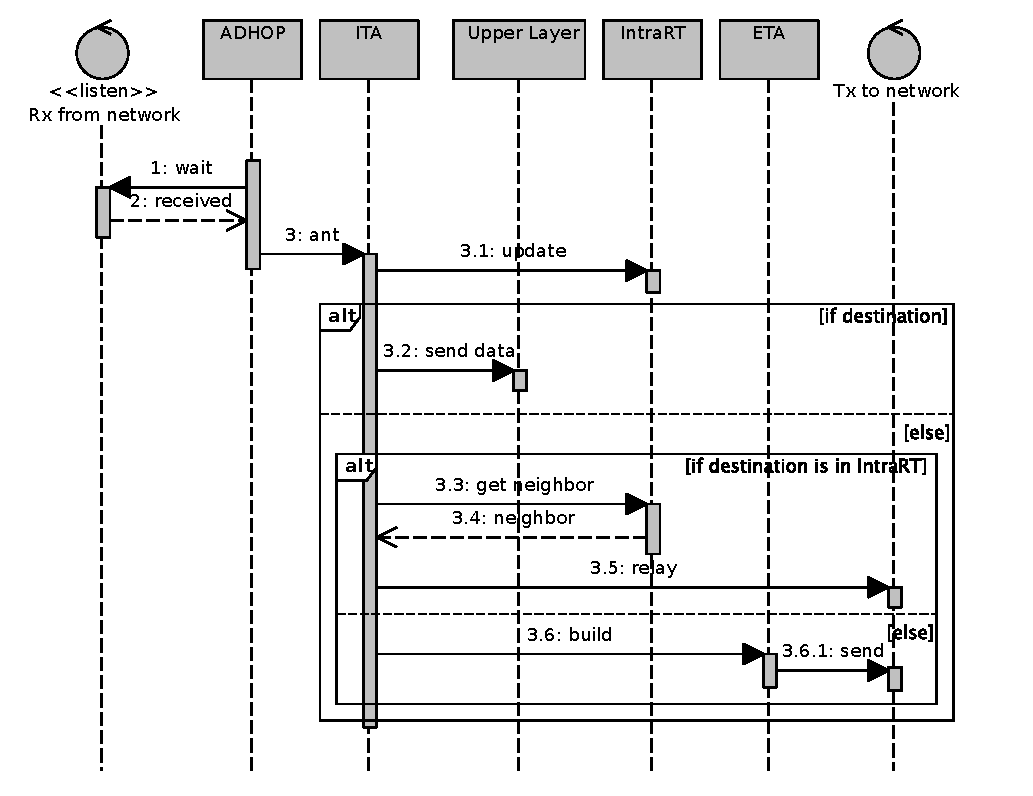
\includegraphics[width=220pt]{fig/adhop_rx_ita.eps}
\caption{FTA Rx}
\label{adhop_rx_ita}
\end{figure}

In each transmissions, the ant selects a node $v_{j}$ as the next hop from the current node $v_{i}$.
At the node $v_{j}$, the ant updates the pheromone $\tau _{i,s}$ on the entry $\left ( v_{i},v_{s} \right )$ in the routing table, where $v_{s}$ is the source node, as follows \cite{Dorigo:2006}:
\begin{equation} \tau _{i,s} = \left ( 1 - \varphi \right ) \cdot \tau _{i,s} + \varphi \cdot \tau _{0} \label{adhop_pheromone_increasing} \end{equation}
where $\tau _{0}$ is the initial value of pheromone, and $\varphi \in \left [ 0,1  \right )$ is the pheromone decay coefficient which is calculated from the heuristic information (Figure \ref{adhop_protocol}) of the node $v_{i}$.

The equation (\ref{adhop_pheromone_increasing}) allows us to diversify the search process by increasing or decreasing the pheromone amount in the routes while allowing other ants to achieve different routes.
It also helps to increase the effect of dynamic hops, allowing us to deal with dynamic network topologies, avoiding possible broken routes, and adapting to the needs of the network through the heuristic information.

The evaporation occurs periodically to all nodes in the network, using the following equation:
\begin{equation} \tau _{i,j} = \left ( 1 - \rho \right ) \cdot \tau _{i,j} , \quad \forall i \in N, \quad \forall j \in Z \label{evaporation} \end{equation}
where $\rho \in \left [ 0,1  \right )$ is the evaporation ratio, $N$ is the set of neighbor nodes, and $Z$ is the set of nodes which, together with neighbor nodes, define entries $\left ( v_{i},v_{j} \right )$ in the routing table.

ADHOP abstracts problems in the network and handles topology changes through pheromone.
It avoids additional overhead in the network as well as possible congestion, avoiding the need to be updated at each change in network topology.
These changes in topology are observed unwittingly by ants.
Thereupon, warning messages or control packets are unnecessary.
It allows us to handle dynamic topologies the way that complex operations in the network can be avoided.

\section{Performance Evaluation}
\label{evaluation}

ADHOP, HOPNET and AODV were analyzed and compared using the \emph{Global Mobile Information System Simulator} (GloMoSim).
It is a protocol simulation software for network systems that supports routing protocols for purely ad hoc wireless networks.
The evaluation took place by way of a number of simulation scenarios.

Each simulation scenario was run for a total of 900 seconds in an environment that is conducive to high data loss.
The nodes were placed randomly in a rectangular area of 700 meters x 400 meters, and each one moved at a maximum speed of 10 meters per second, according to the \emph{Random Way Mobility Model} (RWP).
The data traffic was generated by 20 \emph{Constant Bit Rate} (CBR) sources.
The protocol used for MAC sublayer was the standard IEEE 802.11.
The radio transmission power was set to 15 dBm and the bit rate was 2 megabits per second.
This base scenario was used for the experiments on GloMoSim.
The test scenarios are obtained by varying specific parameters in this base scenario.
The number of nodes ranged from 20 to 200.

Figure \ref{data_delivery_ratio} shows the data packet delivery ratio in this simulation environment.
As the number of node increases, the delivery ratio also increases due to the ants which are able to take the best routes to certain destinations.
If the network is too large and dense, then the delivery ratio is higher due to the large number of routes choices.
On the other hand, if the network is small and sparse, then the delivery ratio decreases due to lack of connectivity among nodes.
Our approach shows better results of data delivery ratio for networks with high scalability and high mobility.
Nevertheless, we notice from the figure that both protocols give a low delivery ratio in the simulations of 100 nodes.
We ascribe it to the congestion, as a result of the placement and mobility of nodes at some point in the simulation.
AODV, a routing protocol for ad hoc networks \cite{Perkins:1999}, shows worse data packet delivery ratio than ADHOP.
However, we can notice that AODV presents better stability in congested conditions.

\begin{figure}[htb]
\centering
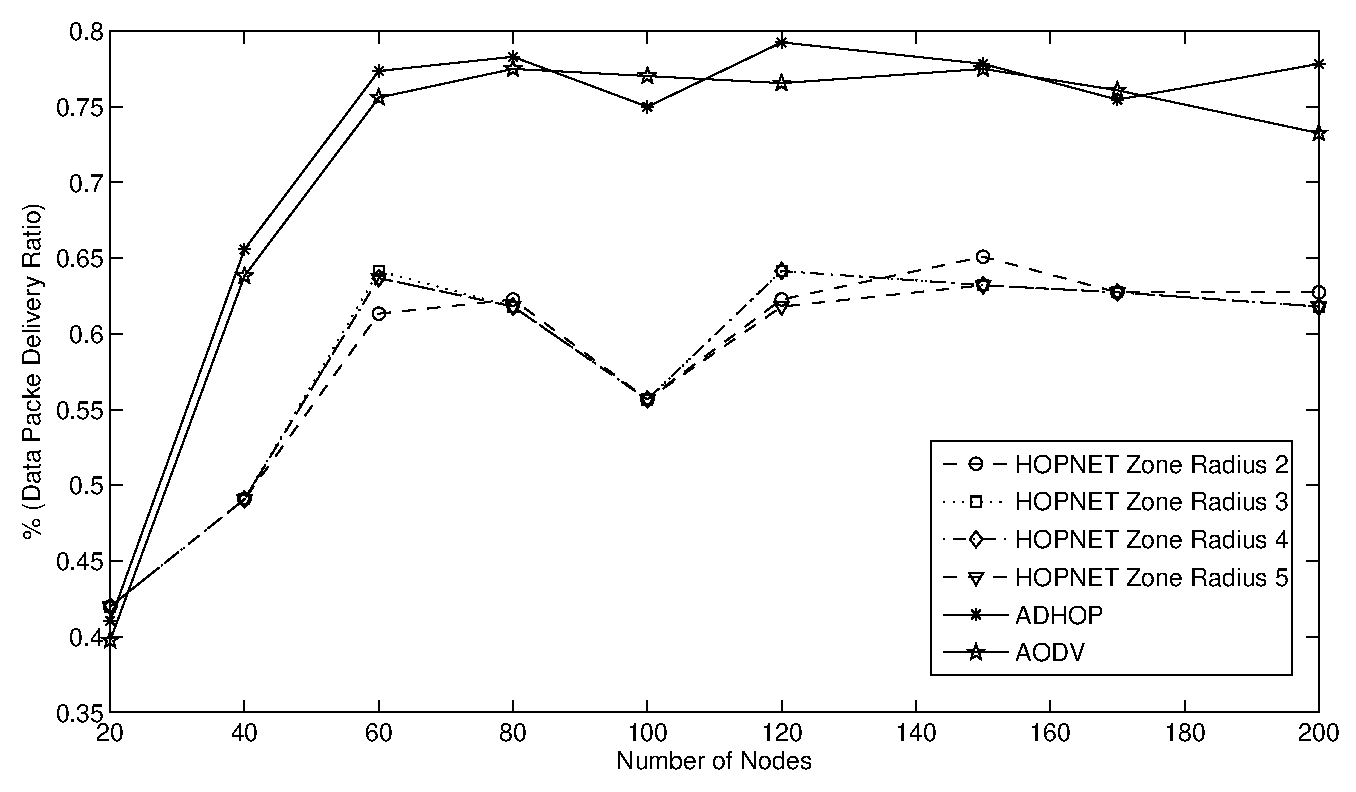
\includegraphics[width=245pt]{fig/data_delivery_ratio.eps}
\caption{Data Packet Delivery Ratio}
\label{data_delivery_ratio}
\end{figure}

Figure \ref{broken_routes} shows the dropped packet ratio due to broken routes.
Because of the low connectivity of small and sparse networks, the data packets cannot be transmitted and the packet loss tends to be low.
Nevertheless, as the number of nodes in the network increases, the amount of broken routes tends to decrease slightly.
Because of the ability of ants to determine the best route between several options to obtain reliable links between nodes along the routes.
Since the routing in ADHOP is solely performed by pheromone, the nodes become more attentive as the topology changes.
It also allows us to use more efficient ways to retrieve a route or discover another (Figure \ref{adhop_rx_ita}).
This way, we can notice that our proposal produces better results of broken routes than HOPNET.

\begin{figure}[htb]
\centering
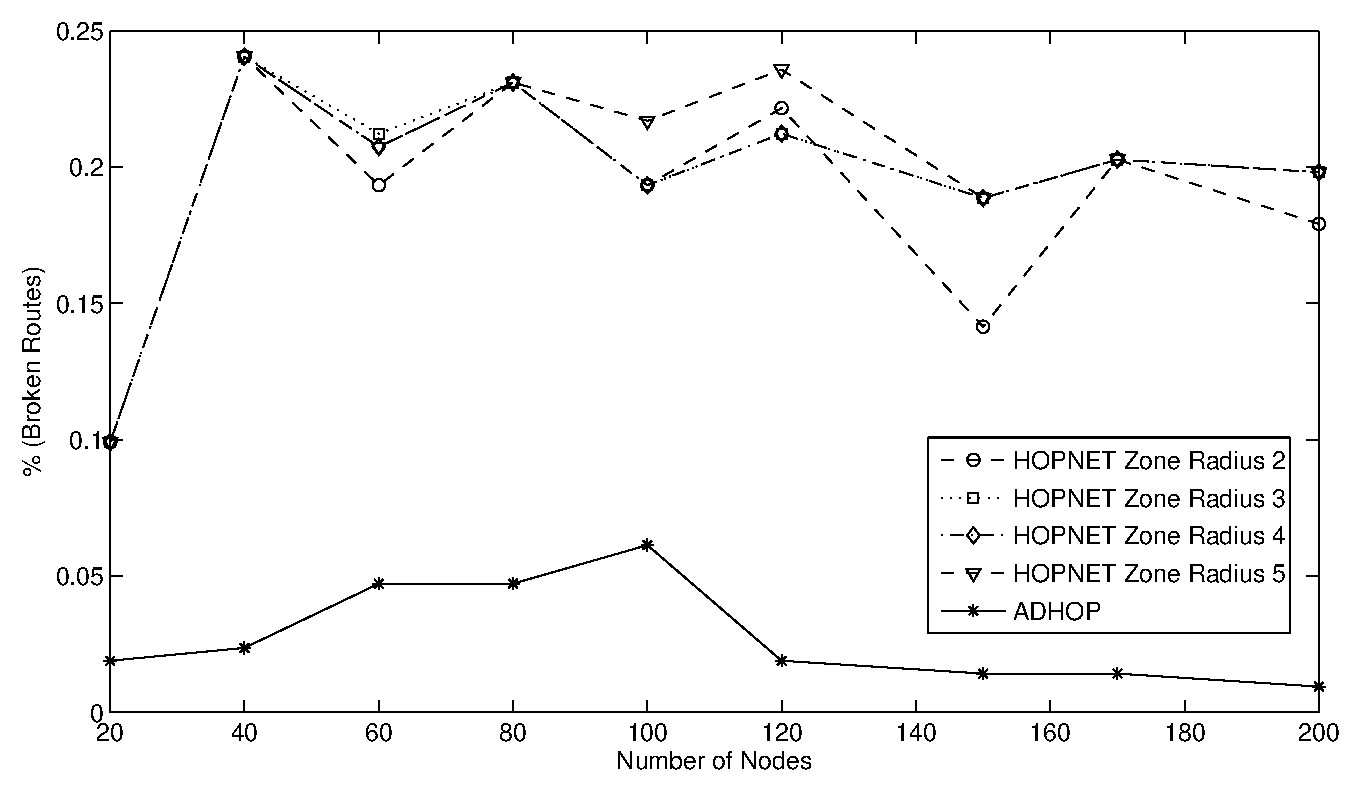
\includegraphics[width=245pt]{fig/broken_routes.eps}
\caption{Broken Routes}
\label{broken_routes}
\end{figure}

Figure \ref{link_failures} shows the results of dropped packets ratio due to link failures.
Different from broken routes, link failures refers to the error messages that originate from MAC sublayer in order to conduct a repair procedure.
We see from the figure that the amount of link failures is superior in small and sparse networks due to low connectivity between nodes.
We also notice that HOPNET produces better results of link failures than ADHOP.
Since our approach is a reactive routing protocol, the links between neighbor nodes tend to be more susceptible to failure.
Because HOPNET has more reliable pheromone information in the zones than ADHOP due to proactive routing.
However, our proposal provides better results in situations of congestion and high mobility due to dynamic hops which provide better adaptability to dynamic topologies than fixed-sized zones.

\begin{figure}[htb]
\centering
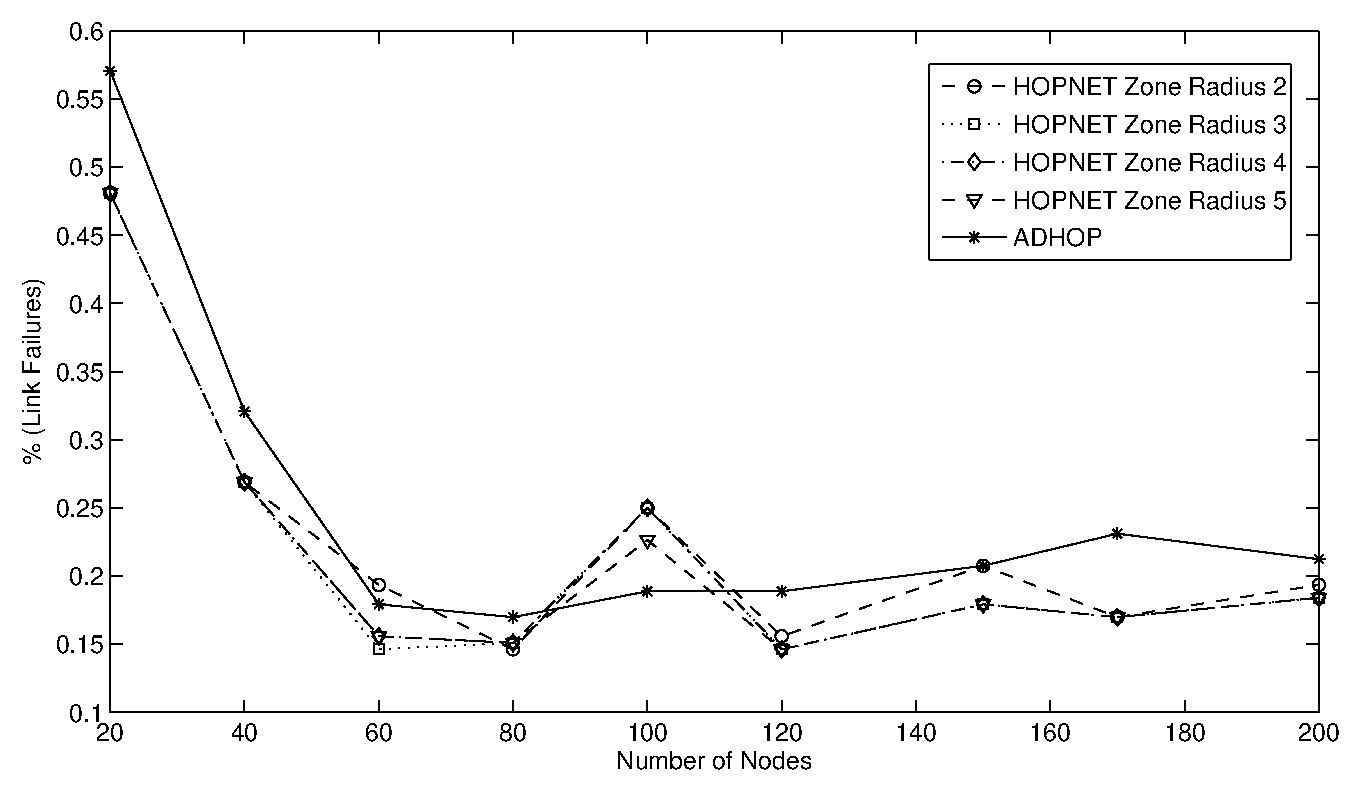
\includegraphics[width=245pt]{fig/link_failures.eps}
\caption{Link Failures}
\label{link_failures}
\end{figure}

Figure \ref{routing_overhead} shows the comparison between HOPNET, ADHOP, and AODV for routing overhead.
AODV presents good results in terms of data packet delivery ratio, as shown in Figure \ref{data_delivery_ratio}.
Route Requests, Route Replies, and Route Errors are the message types defined by AODV.
Considering the high mobility and the high rate of data loss of the simulation performed, AODV has a great load of control packets.
Each time a route breaks, AODV flood the network with these messages to notify and/or define a new route.
In HOPNET, the control packets (ants) are periodically sent out within a zone to maintain the routes in the zone, others are sent out to perform reactive route discovery and repair procedures.
In ADHOP, the data is sent along with the ants thereby decreasing the amount of control packets in the network.
We notice from the figure that ADHOP gives lower routing overhead than HOPNET due to a reduction of ants in the network.
Accordingly, our approach tends to produce low routing overhead for sparse networks due to low connectivity.
However, it also produces high link failures, as explained in the previous figure.
Differently, HOPNET produces high routing overhead for sparse networks.
On this account, it tends to send many more control packets to obtain reliable routes.
And as the number of nodes increases, the routing overhead also tends to increase.
In another way, since the data is sent along with the ants and the routing is reactive, the routing overhead of ADHOP tends to stay almost constant for large and dense networks.

\begin{figure}[htb]
\centering
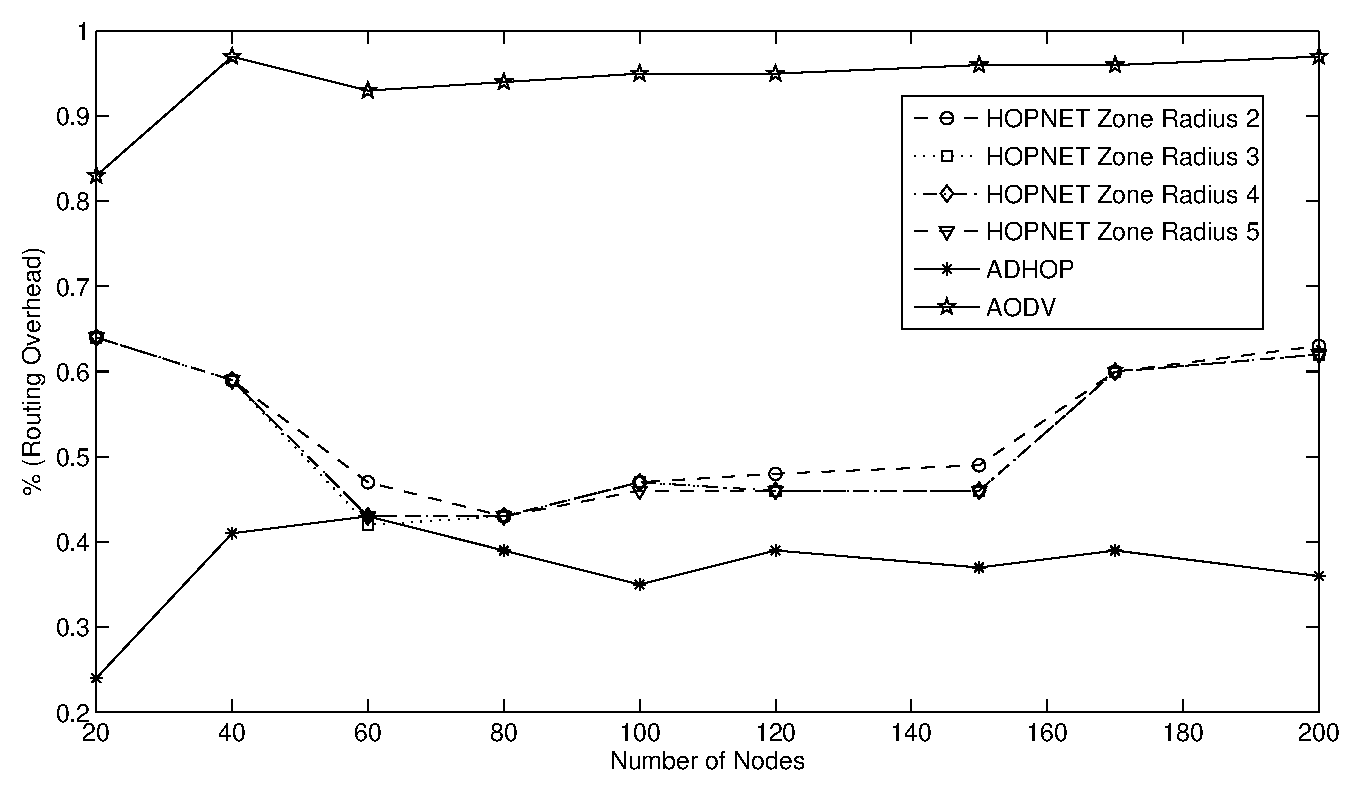
\includegraphics[width=245pt]{fig/routing_overhead.eps}
\caption{Routing Overhead}
\label{routing_overhead}
\end{figure}

\section{Conclusion}
\label{conclusion}

In this paper, we introduce a new routing method based on dynamic hops and present ADHOP, a routing algorithm inspired on HOPNET for dynamic WSNs.
It is a routing algorithm inspired by ACO and uses pheromone as a metric to make routing decisions.
Furthermore, ADHOP uses heuristic information for evaporation and pheromone deposit ratio.
We have evaluated and compared our algorithm to the original HOPNET and obtained better results in terms of data delivery ratio, routing overhead, and congestion avoidance for environments of dynamic topology.
In fact, our study lacks performance evaluation in the context of WSN.
However, our proposal focuses primarily on routing overhead to reduce the amount of control packets from the network to require less effort in communication.
ADHOP achieves these results through the routing method based on dynamic hops which tends to keep the best routes in terms of connectivity without significant losses in the data delivery ratio.
Dynamic hops allow us to improve the routing and to avoid the necessity of complex structures and procedures thus increasing the efficiency and reducing the routing complexity for WSNs.

In future work, we are planning to extend the analysis of our algorithm in WSN environments to improve the experimental scenarios of dynamic topologies.
We also wish to focus on the heuristics information such as location, coverage, and energy consumption.

%\section*{Acknowledgment}
%The authors would like to thank...

\bibliographystyle{IEEEtranS}
\bibliography{paper}

\end{document}

